\documentclass{article}
\usepackage[T1]{fontenc}
\usepackage{lmodern}
\usepackage{graphicx}
\usepackage{amsmath,amssymb}
\usepackage[a4paper,margin=2cm]{geometry}
\usepackage[absolute,overlay]{textpos}
\setlength{\TPHorizModule}{1mm}
\setlength{\TPVertModule}{1mm}
\usepackage[indonesian]{babel}
\usepackage{hyperref}
\setlength{\emergencystretch}{2em}
% unit: Halaman 11

\begin{document}

% === Halaman 11 (python/native) ===

Kriptografi

• Kata cryptography berasal dari bahasa 

Yunani: 


cryptós    (secret or hidden) 


gráphein (writing)

 Artinya “secret writing or “hidden writing”

• Kriptografi: ilmu dan seni untuk menjaga 

keamanan pesan. (Schneier, 1996)

11

Definisi lainnya:

Kriptografi adalah ilmu yang mempelajari teknik-

teknik matematika yang  berhubungan dengan aspek 

keamanan informasi seperti kerahasiaan, integritas 

data, serta otentikasi (Menez, 1996)

% deskripsi: gambar native xref 68
\noindent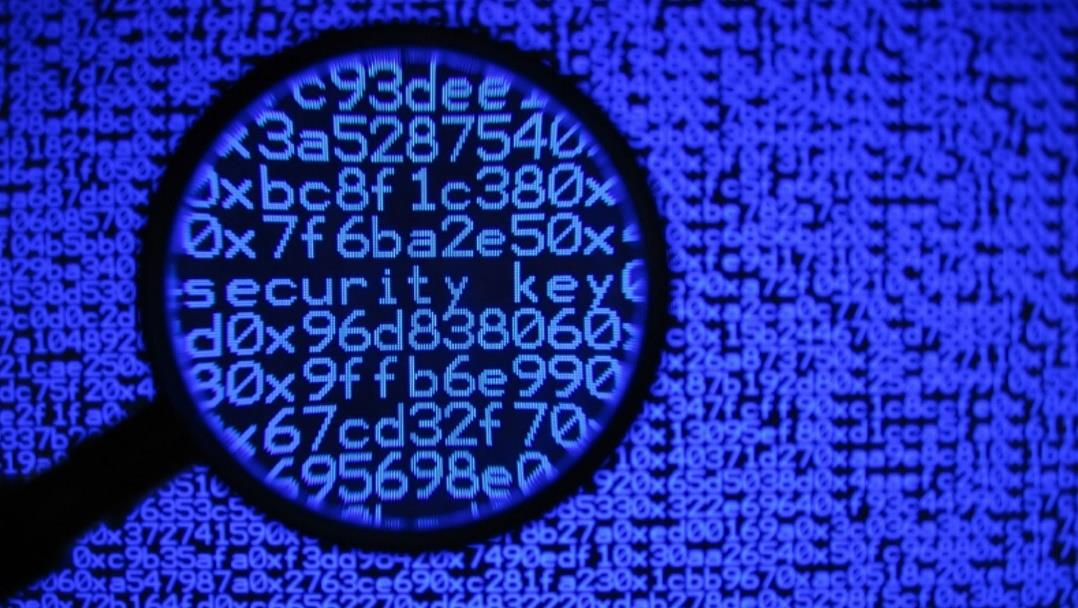
\includegraphics[width=0.85\textwidth]{../../images/python/page_011_img_01.jpeg}

\end{document}
